\documentclass[10pt, a5paper]{article}
\usepackage{pdfpages}
\usepackage{parallel}
\usepackage[T2A]{fontenc}
\usepackage{ucs}
\usepackage[utf8x]{inputenc}
\usepackage[polish,english,russian]{babel}
\usepackage{hyperref}
\usepackage{rotating}
\usepackage[inner=2cm,top=1.8cm,outer=2cm,bottom=2.3cm,nohead]{geometry}
\usepackage{listings}
\usepackage{graphicx}
\usepackage{wrapfig}
\usepackage{longtable}
\usepackage{indentfirst}
\usepackage{array}
\newcolumntype{P}[1]{>{\raggedright\arraybackslash}p{#1}}
\frenchspacing
\usepackage{fixltx2e} %text sub- and superscripts
\usepackage{icomma} % коскі ў матэматычным рэжыме
\PreloadUnicodePage{4}

\newcommand{\longpage}{\enlargethispage{\baselineskip}}
\newcommand{\shortpage}{\enlargethispage{-\baselineskip}}

\def\switchlang#1{\expandafter\csname switchlang#1\endcsname}
\def\switchlangbe{
\let\saverefname=\refname%
\def\refname{Літаратура}%
\def\figurename{Іл.}%
}
\def\switchlangen{
\let\saverefname=\refname%
\def\refname{References}%
\def\figurename{Fig.}%
}
\def\switchlangru{
\let\saverefname=\refname%
\let\savefigurename=\figurename%
\def\refname{Литература}%
\def\figurename{Рис.}%
}

\hyphenation{admi-ni-stra-tive}
\hyphenation{ex-pe-ri-ence}
\hyphenation{fle-xi-bi-li-ty}
\hyphenation{Py-thon}
\hyphenation{ma-the-ma-ti-cal}
\hyphenation{re-ported}
\hyphenation{imp-le-menta-tions}
\hyphenation{pro-vides}
\hyphenation{en-gi-neering}
\hyphenation{com-pa-ti-bi-li-ty}
\hyphenation{im-pos-sible}
\hyphenation{desk-top}
\hyphenation{elec-tro-nic}
\hyphenation{com-pa-ny}
\hyphenation{de-ve-lop-ment}
\hyphenation{de-ve-loping}
\hyphenation{de-ve-lop}
\hyphenation{da-ta-ba-se}
\hyphenation{plat-forms}
\hyphenation{or-ga-ni-za-tion}
\hyphenation{pro-gramming}
\hyphenation{in-stru-ments}
\hyphenation{Li-nux}
\hyphenation{sour-ce}
\hyphenation{en-vi-ron-ment}
\hyphenation{Te-le-pathy}
\hyphenation{Li-nux-ov-ka}
\hyphenation{Open-BSD}
\hyphenation{Free-BSD}
\hyphenation{men-ti-on-ed}
\hyphenation{app-li-ca-tion}

\def\progref!#1!{\texttt{#1}}
\renewcommand{\arraystretch}{2} %Іначай формулы ў матрыцы зліпаюцца з лініямі
\usepackage{array}

\def\interview #1 (#2), #3, #4, #5\par{

\section[#1, #3, #4]{#1 -- #3, #4}
\def\qname{LVEE}
\def\aname{#1}
\def\q ##1\par{{\noindent \bf \qname: ##1 }\par}
\def\a{{\noindent \bf \aname: } \def\qname{L}\def\aname{#2}}
}

\def\interview* #1 (#2), #3, #4, #5\par{

\section*{#1\\{\small\rm #3, #4. #5}}

\def\qname{LVEE}
\def\aname{#1}
\def\q ##1\par{{\noindent \bf \qname: ##1 }\par}
\def\a{{\noindent \bf \aname: } \def\qname{L}\def\aname{#2}}
}

\begin{document}
\title{Data Science for Network Security}
\author{Dmitry Orekhov, Minsk, Belarus\footnote{\url{Dmitry_Orekhov@epam.com}, \url{http://lvee.org/en/abstracts/164}}}
\maketitle
\begin{abstract}
Today network traffic is absolutely out of human control, this is something that human mind cannot manage. On the other hand, network security becomes more and more important, since more and more of human activities are moving to the Network.
The solution could be a software, which is able to learn from past Data incoming, and then to make assumptions about new Data and predictions about the future. Though algorithms for this domain are well-known, there is a problem to implement them, because they are often very resource-consuming. Fortunately, cloud technologies now afford building cheap and productive clusters, and Open Source solutions like Spark provide a powerful tool to build advanced analytics software on top of them.
\end{abstract}
\subsection*{Data collecting}

The first important task for Network Analytics building is a data collection facility. The main idea is to place sensors, which collect statistics data and send it to be collect and analyze.

\begin{figure}[h!]
  \centering 
  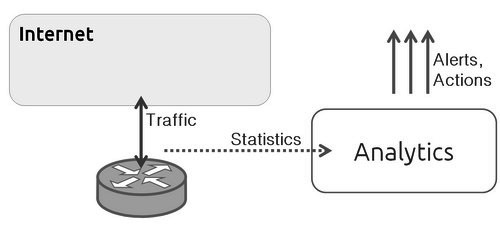
\includegraphics[scale=0.5]{16_2015_fig1}
  
  Fig.1: Statistics collection: the big picture
\end{figure}

\subsubsection*{Sensors}

Sensors are classified by Vantage and Domain. 
\textbf{Vantage} is a place\-ment of sensors within a network. Sensors with different vantages would see different parts of the same events.
\begin{figure}[h!]
  \centering 
  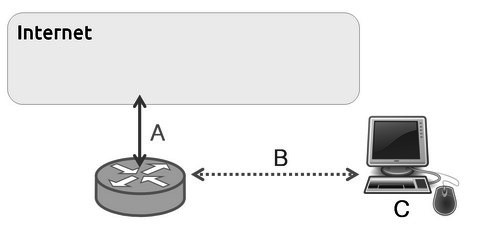
\includegraphics[scale=0.5]{16_2015_fig2}
    
  Fig.2: Vantages
\end{figure}

\textbf{Domain} defines which part of thraffic statistics and metrics to collect. In the other words, it's the information the sensor provides, whether that’s at the host, a service on the host, or the network. Sensors with the same vantage but different domains provide complementary data about the same event. For some events, you might only get informa\-tion from one domain.
\begin{figure}[h!]
  \centering 
  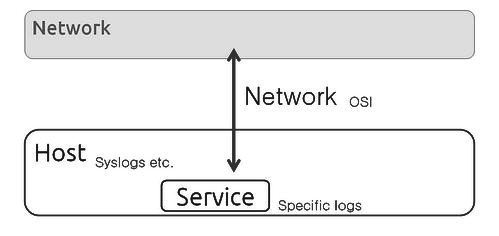
\includegraphics[scale=0.5]{16_2015_fig3}
    
  Fig.3: Domains
\end{figure}

\subsection*{Use Case: DNS Tunneling}

Tunneling -- a mechaninsm to encapsulate low-lewel protocols into high-level protocol.
\begin{figure}[h!]
  \centering 
  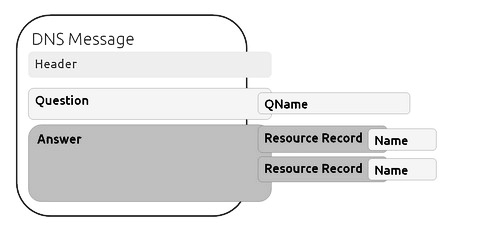
\includegraphics[scale=0.8]{16_2015_fig4}
    
  Fig.4: DNS message, a Big Picture
\end{figure}

In case of DNS tunneling, DNS Resource Records so as Questions may contain Canonical Names; these Names can be easily encoded/de\-coded with Base32 or Base64 methods and can be used to transport unauthorized traffic or botnet protocol commands.

\begin{figure}[h!]
  \centering 
  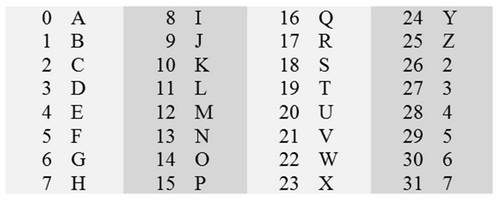
\includegraphics[scale=0.8]{16_2015_fig5}
    
  Fig.5: Base32 encoding
\end{figure}


\subsubsection*{Methods to discover}

\textbf{Payload analysis}

\begin{itemize}
  \item Size of request and response
  \item Entropy of hostnames
  \item Statistical Analysis
  \item Uncommon Record Types
\end{itemize}

\textbf{Traffic analysis}

\begin{itemize}
  \item Volume of DNS traffic per IP address
  \item Volume of DNS traffic per domain
  \item Number of hostnames per domain
  \item Geographic location of DNS server
  \item Domain history
  \item Orphan DNS requests
\end{itemize}

The problem is that the most effective methods to discover DNS traffic demands deep packet inspection. Also, in case of models  based on long-term history, we have to store much statistical data and re-compile the intrusion detection model in a batch job, to be up-to-date.

\subsubsection*{Algorithms}

All algorithms, which could be used for DNS discovering, realate to Machine Learning area; the domain of it is building system, which can be learnt from Data sets and then make predictions about future trends. Today this is very important part of Data Science.

\paragraph{Online algorithms.}

It start with an initial state and analyze each piece of data serially one at a time.

\begin{itemize}
  \item Generally require a chain of Map Reduce jobs
  \item Good fit for Apache Spark, Storm
  \item Primarily batch, good for Lambda architectures
\end{itemize}

\textbf{Example 1: Outlier detection}

\begin{itemize}
  \item Median Absolute Deviation: Telemetry is anomalous if the \linebreak deviation of its latest datapoint
with respect to the median is X times larger than the median of deviations
  \item Standard Deviation from Average: Telemetry is anomalous if the absolute value of the average of the latest three datapoint minus the moving average is greater than three standard deviations of the average.
  \item Standard Deviation from Moving Average: Telemetry is anomalous if the absolute value of the average of the latest three datapoints minus the moving average is greater than three standard deviati\-ons of the moving average.
  \item Mean Subtraction Cumulation: Telemetry is anomalous if the value of the next datapoint in the series is farther than three standard deviations out in cumulative terms after subtracting the mean from each data point
  \item Least Squares: Telemetry is anomalous if the average of the last three datapoints on a projected least squares model is greater than three sigma
  \item Histogram Bins: Telemetry is anomalous if the average of the last three datapoints falls into a histogram bin with less than x
\end{itemize}

\textbf{Example 2: Stream Classification}

\begin{itemize}
  \item Hoeffding Tree (VFDT)
incremental, anytime decision tree \linebreak induction algorithm that is capable of learning from massive data streams, assuming that the distribution generating examples does not change over time
  \item Half-Space Trees
ensemble model that randomly spits data into half spaces. They are created online and detect anomalies by their deviations in placement within the forest relative to other data from the same window
\end{itemize}

The possible topology Big Picture could be like this:
\begin{figure}[h!]
  \centering 
  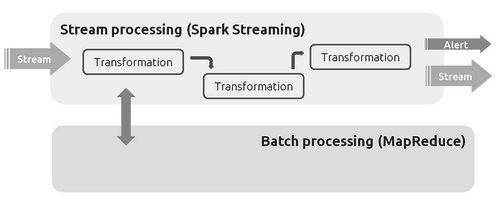
\includegraphics[scale=0.8]{16_2015_fig6}
    
  Fig.6: Online algorithms, Topology
\end{figure}

\paragraph{Offline algorithms.}

It analyzes entire data set at once.

\begin{itemize}
  \item Generally a good fit for Apache Hadoop/Map Reduce
  \item Model compiled via batch, scored via stream processor
\end{itemize}

\textbf{Example: Hypothesis Tests}

\begin{itemize}
  \item Chi2 Test (Goodness of Fit): A feature is anomalous if the data for the latest micro batch (for the last 10 minutes) comes
from a different distribution than the historical distribution for that feature
  \item Grubbs Test: telemetry is anomalous if Z score is greater than the Grubb's score.
  \item Kolmogorov-Smirnov Test: check if data distribution for last 10 minutes is different from last hour
  \item Simple Outliers test: telemetry is anomalous if the number of outliers for the last 10 minutes is statistically different then the
historical number of outliers for that time frame
\end{itemize}

Also, some other types of algorithms can be used

\begin{itemize}
  \item Decision Trees/Random Forests
  \item Association Rules (Apriori)
  \item Auto Regressive (AR) Moving Average (MA)
\end{itemize}

In fact, at using Offlimne algorithms, all analysis is performed as batch tasks, the Streaming part just applies rules compiled by the Batch part. A possible topology Big Picture could be like this
\begin{figure}[h!]
  \centering 
  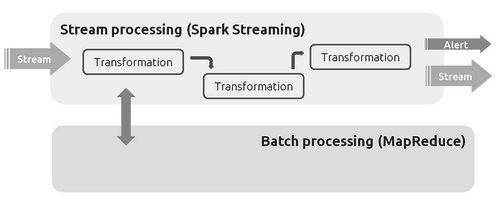
\includegraphics[scale=0.8]{16_2015_fig7}
  
  Fig. 7: Offline algorithms, Topology
\end{figure}

\subsubsection*{Technology stack: everything Free}

It's very important, that all software to build Analytics based on Machine Learning so as for Data storage is Free/Libre one. All solutions which we are using are publiched under Apache 2.0, MIT and so on.
For Streaming part it was used Spark Streaming and Spark for Batch jobs as well. Message Queues which we are using are Kafka and RabbitMQ.

\end{document}
